%\documentclass[11pt]{article}  % for e-submission to ApJ
\documentclass[11pt]{NSF}  % for e-submission to ApJ


\usepackage{graphicx, natbib, color, bm, amsmath, epsfig}
\usepackage{wrapfig}

%paper commands, for when not using aastex
\newcommand\physrep{Phys.~Rep.}
\newcommand\fcp{Fund.~Cosmic~Phys.}
\newcommand{\pre}{Phys Rev E}
\newcommand{\apj}{ApJ}
\newcommand{\apjs}{ApJS}
\newcommand{\aj}{AJ}
\newcommand{\aap}{A\&A}
\newcommand{\mnras}{MNRAS}
\newcommand{\araa}{ARA\&A}
\newcommand{\procspie}{Proc.SPIE}
\newcommand{\pasj}{PASJ}
\newcommand{\iaucirc}{IAU Circ.}
\newcommand{\aplett}{AP Letters}
\newcommand{\aaps}{AAPS}
\newcommand{\aapr}{AAPR}
\newcommand{\nat}{Nature}
\newcommand{\apjsupp}{ApJS}
\newcommand{\pasp}{PASP}
\newcommand{\apjl}{ApJL}
\newcommand\prl{Phys.~Rev.~Lett.}
\newcommand\apss{Ap\&SS}




%%%% PUT NEW COMMANDS AND DEFINITIONS HERE %%%%
\usepackage{graphicx, natbib, color, bm, amsmath, epsfig}

%
% Hijacked and hacked from aastex.cls
%
%\def\newblock{\hskip .11em\@plus.33em\@minus.07em}%

%\newcommand\plotone[1]{%
% \typeout{Plotone included the file #1}
% \centering
% \leavevmode
% \includegraphics[width={\eps@scaling\columnwidth}]{#1}%
%}
%\newcommand\plotone[1]{
% \includegraphics[width=3.0in]{#1}%
%}
%\let\tableline=\hline
%enzo commands
\newcommand\jcompphys{J.~Comput.~Phys}
\newcommand\physfluidsa{Phys.~Fluids~A}
\newcommand\physfluids{Phys.~Fluids}
\newcommand\physlettA{Phys.~Lett.~A}
\newcommand\jfm{J.~Fluid~Mech.}
\newcommand\ccm{Comput.~Phys.~Commun.}
\newcommand\jphysique{J.~Physique~I}
\newcommand\revmodphys{Rev.~Mod.~Phys.~}

%\newcommand\aap{\ref@jnl{A\&A}}% 
%\newcommand\prb{\ref@jnl{Phys.~Rev.~B}}% 
          % Physical Review B: Solid State 


\newcommand{\ratio}{\mathcal{R}}
\newcommand{\yt}{{\tt yt}}
\newcommand{\Lmax}{\ell_{\rm max}}
\newcommand{\enzo}{{\small Enzo}}
\newcommand{\menzo}{{EnzoMHD}}
\newcommand{\Menzo}{{EnzoMHD}}
\newcommand{\zeus}{{\small ZEUS}}
\newcommand{\Lbox}{L_{\rm box}}
\newcommand{\Nroot}{N_{\rm root}}
\newcommand{\K}{\,\rm K}
\newcommand{\dave}{DaveThena}
\newcommand{\grid}{{\tt grid}}

%\newcommand{\lct}[3]{\ensuremath{\epsilon_{#1,#2,#3}}}
\newcommand{\lct}[1]{\ensuremath{\epsilon_{#1}}}
%grid location commands.
\newcommand{\iph}{i + \frac{1}{2}}
\newcommand{\imh}{i - \frac{1}{2}}
\newcommand{\jph}{j + \frac{1}{2}}
\newcommand{\jmh}{j - \frac{1}{2}}
\newcommand{\kph}{k + \frac{1}{2}}
\newcommand{\kmh}{k - \frac{1}{2}}

\newcommand{\ipmh}{i \pm \frac{1}{2}}
\newcommand{\half}{\frac{1}{2}}
\newcommand{\quart}{\frac{1}{4}}
\newcommand{\tquart}{\frac{3}{4}}

%physics commands
\newcommand{\avir}{\ensuremath{\alpha_{\rm{vir}}}}
\newcommand{\mach}{\ensuremath{\mathcal{M}}}
\newcommand{\hmag}{\ensuremath{H_{\rm{M}}}}
\newcommand{\alfmach}{\ensuremath{\mathcal{M_{\rm{A}}}}}
%\newcommand{\msun}{\ensuremath{\rm{M}_\odot}}
\newcommand{\msun}{\ensuremath{M_\odot}}
\newcommand{\lsun}{\ensuremath{L_\odot}}
\newcommand{\rsun}{\ensuremath{R_\odot}}

\def\mch{\ensuremath{M_{\rm{Ch}}}}
\def\AD{{\rm{AD}}}

%math commands
\def\rms{\ensuremath{\rm{rms}}}
\newcommand{\pts}[1]{\emph{(#1 pts)}}
\newcommand{\dbd}[2]{\frac{ \partial #1 }{ \partial #2} }
\newcommand{\ddbd}[2]{\frac{ d #1 }{ d #2} }
\newcommand{\dDbD}[2]{\frac{ \mathrm{D} #1 }{ \mathrm{D} #2} }
\newcommand{\curl}{\nabla \times}
\newcommand{\divb}{\ensuremath{\nabla \cdot {\bvec}}}
\newcommand{\divv}{\ensuremath{\nabla \cdot {\vvec}}}
\newcommand{\divbo}{$\nabla \cdot {\bf B} = 0$}
\newcommand{\intd}[1]{\int_#1^{#1 + \Delta #1} }
\newcommand{\dt}{\Delta t}
\newcommand{\dx}{\Delta x}
\newcommand{\dy}{\Delta y}
\newcommand{\dz}{\Delta z}
\newcommand{\p}[1]{#1^\prime }
\newcommand{\pp}[1]{#1^{\prime \prime} }
\newcommand{\tff}{\ensuremath{t_{\rm{ff}}}}
\newcommand{\kkmin}{\ensuremath{k/k_{\rm{min}}}}
\newcommand{\kmax}{\ensuremath{k_{\rm{max}}}}

%dcc color commands
\definecolor{orange}{rgb}{1.        ,  0.54,  0}
\newcommand{\orange}[1]{\textcolor{orange}{#1}}

\newcommand{\gtt}[1]{\textcolor{green}{{\tt#1}}}
\newcommand{\red}[1]{\textcolor{red}{#1}}
\newcommand{\yellow}[1]{\textcolor{yellow}{#1}}
\newcommand{\blue}[1]{\textcolor{blue}{#1}}
\definecolor{meta}{rgb}{0.371,0.617,0.625} %cadet blue for
                                           %non-production worthy
                                           % discussion of the work
\newcommand{\meta}[1]{\textcolor{meta}{#1}}
\newcommand{\green}[1]{\textcolor{green}{#1}}
\newcommand{\aake}[1]{\textcolor{blue}{#1}}
\newcommand{\bld}[1]{\mathbf{#1}}

\def\here{\red{notes later}}
%\newcommand{\hilite}[1]{\textcolor{red}{#1}}
%\newcommand{\hilite}[1]{#1}

%\newcommand{\bold}[1]{{\bf #1}}
%the comment maker, dc: the first one will show all comments in green, 
%the second hides them all.
%\newcommand{\dc}[1]{\textcolor{green}{#1}}
\newcommand{\dc}[1]{}
%\newcommand{\dc}[1]{#1}
%\def\bvec{\ensuremath{\vec{B}}}
%\def\vvec{\ensuremath{\vec{v}}}
\def\Bvec{\ensuremath{{\bf B}}}
\def\Jvec{\ensuremath{{\bf J}}}
\def\Avec{\ensuremath{{\bf A}}}
\def\bvec{\ensuremath{{\bf b}}}
\def\vvec{\ensuremath{{\bf v}}}
\def\uvec{\ensuremath{{\bf u}}}
\def\rvec{\ensuremath{{\bf r}}}
\def\xvec{\ensuremath{{\bf x}}}
\def\kvec{\ensuremath{{\bf k}}}
\def\Omegavec{\ensuremath{{\bf \Omega}}}
\def\omegavec{\ensuremath{{\bf \omega}}}
%\newcommand{\BlockOut}[1]{}
\newcommand{\BlockOut}[1]{#1}
\newcommand{\imp}{\ensuremath{\implies}}
\newcommand{\question}[1]{\textcolor{red}{#1}}
\definecolor{pink}{rgb}{1.        ,  0.75294118,  0.79607843}
\definecolor{maroon}{rgb}{0.69019608,  0.18823529,  0.37647059}
\newcommand{\ToRead}[1]{\textcolor{maroon}{#1}}
\newcommand{\ToReadUrgent}[1]{\textcolor{red}{#1}}
\newcommand{\HaveRead}[1]{\textcolor{black}{#1}}
\newcommand{\Old}[1]{\textcolor{blue}{#1}}
\newcommand{\Scanned}[1]{\textcolor{meta}{#1}}
\newcommand{\dccnote}[1]{}
%\newcommand{\dccnote}[1]{\textcolor{red}{#1}}
\def\nn{\nonumber}

\newcommand{\get}[1]{\textcolor{red}{#1}}
\definecolor{gray}{rgb}{0.5,0.5,0.5}
\newcommand{\gray}[1]{\textcolor{gray}{#1}}
\newcommand{\clean}[1]{\textcolor{gray}{#1}}
\newcommand{\ToDo}[1]{\textcolor{red}{#1}}
\def\etal{{\sl et al.}}

%chemistry commands
\newcommand{\Htwo}{\ensuremath{\rm{H}_2}}
\newcommand{\twelveco}{\ensuremath{^{12}\rm{CO}}}
\newcommand{\thirteenco}{\ensuremath{^{13}\rm{CO}}}

\newcommand{\mhdlabel}{{_{MHD}}}
\newcommand{\gravlabel}{{_{Grav}}}
\newcommand{\fclabel}{{_{fc}}}
\newcommand{\explabel}{{_{exp}}}
\newcommand{\sci}[1]{\ensuremath{\times {10^{#1}}}}
\newcommand{\percc}{\ensuremath{\rm{cm}^{-3}}}
\newcommand{\gcc}{\ensuremath{\rm{g}\ \rm{cm}^{-3}}}
\newcommand{\kms}{\ensuremath{\rm{km}\ \rm{s}^{-1}}}
\newcommand{\cms}{\ensuremath{\rm{cm}\ \rm{s}^{-1}}}
\newcommand{\cmperg}{\ensuremath{\rm{cm}^{2}\ \rm{g}^{-1} }}
\newcommand{\cmcmpers}{\ensuremath{\rm{cm}^2\ \rm{s}^{-1} }}
\def\muG{\ensuremath{\mu\rm{G}}}
\def\micron{\ensuremath{\mu\rm{m}}}
\def\alf{Alfv\' en}
\def\Alfvenic{Alfv\' enic}
\def\sa{super-Alfv\' enic}
\def\Sa{Super-Alfv\' enic}
\def\suba{sub-Alfv\' enic}
\def\Suba{Sub-Alfv\' enic}
\def\transa{trans-Alfv\' enic}
\def\Transa{Trans-Alfv\' enic}
\def\cs{\ensuremath{c_{\rm{s}}}}
\def\va{\ensuremath{v_{\rm{A}}}}
\def\sfrff{\ensuremath{{\rm SFR_{ff}}}}
%\def\velocity{\ensuremath{\vec{v}}}
%\def\magnetic{\ensuremath{\vec{B}}}
\def\velocity{\ensuremath{{\bf v}}}
\def\magnetic{\ensuremath{{\bf B}}}
\newcommand{\Fourier}[1]{\ensuremath{\tilde{#1}}}
\def\hfw{0.49}
\def\hw{0.49}
\def\fw{0.9}

\def\ssp{\def\baselinestretch{1.0}\large\normalsize}

\def\rhoc{\ensuremath{\rho_{\rm{c}}}}
\def\erf{\ensuremath{\rm{erf}}}


\def\SUtotal{2.9\sci{5}       }%cut from table1.
\def\tfinal{T_{\rm{final}}}
\def\suzu{\ensuremath{\rm{SU}_{\rm{zu}}}}
\def\nzones{N_{\rm{z},\ell}}
\newcommand{\Lund}{\ensuremath{\mathrm{S}}}
%\newcommand{\SUestimate}[1]{\textcolor{red}{#1}}
\newcommand{\SUestimate}[1]{#1}
\def\SUtotal{1.6\sci{5}       }                                                       
%\def\SUturb{1.8\sci{4}}
%\def\SUcore{1.2\sci{4}}
%\def\SUcmb{2.6\sci{4}}
%\def\SUgal{2.2\sci{3}}
%\def\DiskTurb{5.6\sci{3} Gb}
%\def\DiskCore{1.6\sci{5} Gb}
%\def\Diskcmb{1.7\sci{4} Gb}
%\def\Diskgal{1.1\sci{4} Gb}
%\def\StoreTotal{1.9\sci{5} Gb}
\def\nameTurbulence{\emph{turbulence}}
\def\nameTurbShort{\emph{turb}}
\def\nameCores{\emph{cores}}
\def\nameCMB{\emph{foregrounds}}
\def\nameGalaxies{\emph{galaxies}}
\def\suPerZoneUpTurbulence{\ensuremath{2.0\sci{-11}}}
\def\suPerZoneUpCores{\ensuremath{6.2\sci{-11}}}
\def\suPerZoneUpCMB{\ensuremath{6.2\sci{-11}}}
\def\suPerZoneUpGalaxies{\ensuremath{3\sci{-10}}}

\citestyle{aa}  % correct formatting for ApJ style files

\usepackage{aas_macros}
\begin{document}

\begin{centering}
\begin{LARGE}
%  Scaling Information for 
    Three Projects in Astrophysical Magnetohydrodynamics
\end{LARGE}


\vspace{2mm}
{\bf PI: David C. Collins} (Florida State University)

\end{centering}
\pagestyle{plain}

%\red{TO DO}
%`` Note that the proposal appears hastily put together, with typographical
%errors throughout.''
%
%``The authors neglected to provide specific information on how the runs would be
%setup. This must be included in future proposals or they may be rejected.''
%
%`` However, the most important information is missing (or at least I could not
%find it): How many cores will be used during the proposed calculations? Without
%this information the scaling plot is not very useful, and particularly the
%'effective use of resources' cannot be judged properly. ''
%
%``For now I recommend to award 50\% of the request, which will allow the group to
%start with the parameter study. Scarce resources will also encourage the group
%to prune the parameter list after initial results roll in. ''
\tableofcontents
%\input{abstract}       %dcc todo 2022
\section{Introduction}
\label{sec.intro}

We are requesting \SUtotal\ SUs on Stampede 2 for the period beginning June 1,
2022.  This allocation will support four projects involving astrophysical
magnetic fields and turbulence.  The first project (\nameTurbulence) explores analytical
formulae we have developed for isothermal turbulence, which is relevant for many
astrophysical processes, among them the formation of stars.  The second project
(\nameCores) simulations the formation of pre-stellar cores from low density
interstellar clouds.  The third project (\nameCMB) examines the polarized signal
produced by the interstellar medium, which is in the way of our understanding of
the cosmic microwave background (CMB). The fourth projcet (\nameGalaxies)
simulates entire galaxies, in order to understand the growth of the magnetic
field.
This research is supported by two NSF grants.  The first two projects
(\nameTurbulence\ and \nameCores)  
are
supported by NSF AST-1616026, and the third (\nameCMB) is supported by 
NSF AST-2009870.
We are hopful that the \nameGalaxies\ project will be funded by a pending
proposal.


These projects support three graduate students.  Luz Jimenez Vela is working on
the \nameCores\ project; Branislav Rabatin is working on the \nameTurbulence\
and \nameCMB\ projects; and Jacob Strack is working on the \nameGalaxies\
project.


Table \ref{table1} shows the cost for each project.  Each of the four projects
uses a slightly different physics package, which affects  the cost of the
simulation.  In addition, two of the four projects employ adaptive mesh
refinement (AMR), a technique that adaptively changes the resolution of the
simulation.  This also affects the cost of the simulation.

In Section
\ref{sec.background} we motivate each project and describe the simulations to be
run.  In Section \ref{sec.method} we
describe the compuational tools to be used.  In Section \ref{sec.plan} we
give the projected cost  and disk usage of these simulations.

    %dcc todo 2022
\section{Scientific Background}
\label{sec.background}

Here we will introduce the physical motivation for the projects, and describe
the simulations to be performed.  Detailed accounting of the performance and
simulation structure can be found in Section \ref{sec.plan}.  


\subsection{Background: Turbulent Energy}
\label{sec.back_turb}
Turbulence is ubiquitous in astrophysical processes.  We have developed analytic
predictions for the distribution of energies in isothermal turbulence, both
supersonic and subsonic. These simulations will verify our analytic predictions,
and examine if deviations seen in preliminary studies are due to lack of
resolution or interesting physics.
We provide the background for the \nameTurbulence\ project in Section
\ref{subsec.turb_motivate},
and motivate the simulations that support this study in Section
\ref{subsec.turb_sims}.


\subsubsection{Motivation: \nameTurbulence}
\label{subsec.turb_motivate}

The interstellar medium (ISM) is the gas between stars in the galaxy.  It cools
very effectively, so can be treated as isothermal \red{Krumholz star formation
book}.  The ISM is also turbulent, with supersonic shocks driven by supernovae
causing supersonic turbulence throughout the interstellar medium.  This
turbulence impacts the formation of stars (see Section \ref{sec.back_cores}) and
causes a polarized screen that is blocking our view of the light from the big bang (see
Section \ref{sec.back_foregrounds}), among many other effects
\citep{Elmegreen04}. It is also interesting in its own right.  We have developed
analytic formulae for the probability density function (PDF) of internal energy
and kinetic energy, as well as their joint distribution.  In this project we
will verify these formulae with high resolution simulations.

Supersonic turbulence is compressible, and the distribution of density
fluctuations is described by a log normal, i.e. the log of density is
distributed as a gaussian.  The distribution of velocity is roughly Maxwellian,
i.e. each of the three velocity components is a guassian, and added in quadrature the
distribution is Maxwellian.  
We have recently found analytic distributions for the internal energy and
kinetic energy, as well as their joint
distribution.   Kinetic energy is defined in the familiar way, $E_K=\half \rho
v^2$.  Internal energy is defined as $E_T= c_s^2 \rho \ln \rho/\rho_0$, where
$c_s$ is the sound speed and $\rho_0$ is the mean density.  The joint
distribution of these two quantities can be seen in Figure \ref{fig.energy},
along with our analytic prediction (dotted lines).
Each panel shows the joint PDF of $E_K$ and $E_T$;  the color field shows the
PDF derived from data; the solid lines show logarithmically spaced contours of
the data; the dashed lines show the theoretical prediction.  The first panel is
subsonic, with $\mach=0.5$, the middle has $\mach=1$, and the third panel is
slightly supersonic, with $\mach=2$.  Significant changes in the behavior of the
distribution, with high $K_E$ gas developing along side high $E_T$ gas, are both
predicted by the analytical dashed lines and seen in the data.

These energy distributions will be useful
in future studies of turbulence in the ISM, as the energetics of the gas
determine, e.g., what can collapse to form stars.  

\subsubsection{Simulations: \nameTurbulence}
\label{subsec.turb_sims}

Our preliminary simulations were run with a modest resolution of $256^3$.  This
is enough to find reasonable agreement, but imperfect. This can be seen most
easily in the first panel of Figure \ref{fig.energy}, by examining the center
most (red) contours. The solid line shows simulation, while the dashed line
shows theory, which clearly agrees, but only approximately.  This lack of
agreement can be one of several things, the first to examine is numerical
resolution.  With insufficient resolution, energy is transferred from large to
small scales faster than would be natural, which could be why we have mediocre
agreement in our predicted theory.  The proposed simulations will quadruple this
resolution to $1024^3$.  Owing to the substantial evolution with Mach number, we
will run some subsonic cases (\mach=0.5, 1.0) and some moderate and highly
supersonic cases (\mach=2,4,7).  The driving is done with the \red{OU get
citation}


\subsection{Background: Star Formation}
\label{sec.back_cores}

The formation of stars is filled with filamentary, fractal structures
\citep{Andre14}.  The
\nameCores\ project will study the behavior of collapsing gas as it transitions
from fractal structures to form dense prestellar cores.  We will motivate the
study in Section \ref{subsec.cores_motivate}, and describe the simulations
in \ref{subsec.cores_sims}.


\subsubsection{Motivation: \nameCores}
\label{subsec.cores_motivate}
The formation of stars is one of the most important processes in astrophysics,
as stars provide most of the light we see in the night sky, and they produce the
energy and metal
that dictates the structure and composition of a galaxy.  
A \emph{prestellar core} is a knot of dense gas
formed by gravity in a molecular cloud, which will ultimately form a star.  The
formation of these cores is one of the more difficult puzzles in star formation,
as it is fundamentally dictated by chaotic dynamics of the turbulence in the
cloud.  This is the focus of the \nameCores\ project.

One of our previous studies (Collins et al 2022, in prep) examined the collapse of a molecular cloud by
including semi-Lagrangian tracer particles that follow the flow.  The particles
that are found in dense cores at the end of the simulation are then followed
backwards in time to 
to examine the \emph{preimage} of the gas, before it collapses.  This will allow
us to better constrain star formation models.  

One of the curious findings is the fractal nature of the preimage gas.  We find
that gas from distinct cores at the end of the simulation begins life mixed with
one another in a fractal manner. This can be seen in Figure
\ref{fig.cores}, which shows the overlap of a collection of preimages at the
beginning of the simulation in the first 3 panels, and the
collapse to form dense cores in the fourth.  The length scale in the first three panels translates to
roughly 2 pc in size.  These panels show the overlap and fractal, filamentary nature of
the gas before it collapses.  The
last panel shows the un-mixing of the gas as it collapses in time.

\subsubsection{Simulations: \nameCores}
\label{subsec.cores_sims}

The simulation presented in Figure \ref{fig.cores} was one of a suite of three
simulations with varied magnetic field strength.  We began with fully developed
turbulence, and then added tracer particles and turned on gravity and AMR.  These simulations were
relatively low resolution as we developed the analysis techniques and learned
about extended nature of the primage gas.
Our proposed simulations will greatly improve the resolution
to explore if these structures are in fact fractal, or a result of low
resolution. The size of the box is 5 pc, and the r.m.s. Mach number is 9.  They
will begin from existing simulation data.  The target simulations will have $512^3$ root grid and 4 levels of
AMR, and $1024^3$ particles.  This is an increase of 4 in linear scale for the
gas, and 16 for the particles over the results shown in Figure \ref{fig.cores}.
The proposed suite of three simulations will mirror the magnetic field strengths
of the preliminary studies.  The simulations will be similar to those presented
in \citep{Collins12}, but with tracer particles and sinks.
It will run for a total of one free-fall time, where $t_{ff}=(G
\rho)^{-1/2}=1$Myr.  Here
$G$ is the gravitational constant, and $\rho$ is the mean density of the box.
These simulations will utilize isothermal MHD, gravity, and particle solvers.



\subsection{Background: Galaxies}
\label{sec.back_galaxies}
The galactic magnetic field can be seen in Figure \ref{fig.planck}.  This figure
is an all-sky projection of dust in the galaxy, seen at 353 GHz by the Planck
satellite, smeared along the direction of
the magnetic field.  Our goal in the \nameGalaxies\ project is to understand the
origin of this magnetic field.  We will discuss the background in Section
\ref{subsec.galaxies_motivate}, and describe the simulations we will perform in
Section \ref{subsec.galaxies_sims}

\subsection{Motivation: \nameGalaxies}
\label{subsec.galaxies_motivate}

It is well know that the Milky Way has a large scale magnetic
field of roughly $\sim 5 \mu$G, about 200,000 time weaker than a refrigerator
magnet, but spanning the entire galaxy.   

The origin of this magnetic field is an open question.  There are presently two
known \emph{dynamos}, that is mechanisms to amplify magnetic fields. They differ in
two ways; the length scales over which they act, and the time scales over which
they act.  The fast
dynamo converts turbulent kinetic energy to magnetic energy at small scales, and
produces disordered fields quickly.  The slow dynamo produces large scale fields
slowly, with large scale convective motions. The magnetic field in the Milky Way, as well as other similar galaxies,
shows large scale order, but based on observations of galaxies, must have been
built up quickly. 

The magnetic field in the Galaxy is largely in one direction, losely following
the spiral arms.  On the way to producing a large scale magnetic field, both
dynamo mechanisms produce a
substantial amount of field in all directions.  Thus to have a field of mostly
one direction, the other directions must be expelled from the galaxy.
(Selectively eliminating one component of magnetic field is not possible at
these scales.)
Thus the buoyancy of the gas as
it leaves the face of the disk is important in setting the rate of growth of
the mean field.  Like many problems in physics, the answer depends sensitively
on boundary conditions.

The circum-galactic medium (CGM) is the gas that's outside disk the galaxy, but still
bound to it.  It is extremely hot (millions of Kelvin) and extremely low density
(0.1 $cm^{-3}$) and thus unfortunately difficult to observe.
The purpose of this project is to examine the growth of magnetic fields in Milky
Way sized galaxies.  
Specifically, to examine the impact of the circum-galactic
medium (CGM) properties on the dynamo. We expect that an ordered field within
the disk requires a buoyant CGM, that is gas that is expelled from the galaxy by
supernovae continues to rise, rather than falling back down immediately.  

\subsection{Simulations: \nameGalaxies}
\label{subsec.galaxies_sims}

Our proposed simulations will begin at very large scale, $1.3$ Mpc.  This is to
separate the boundary from the region of interest, and to give the CGM a large
enough volume to expand.  We will resolve a nest of refinement grids, each one
1/2 of its parent grid on a side, giving constant number of zones per level.
This will be done for 5 levels.  We will allow the simulation to 
refine for a further 4 levels, based on the local density of the gas.  Nine
levels then gives us 10pc of resolution on the finest
level, so we will resolve molecular clouds by a few zones.  We will have ample
resolution in the disk to study the dynamo action as it occurs, and sufficient
resolution in the CGM to serve as an appropriate boundary.  As we are simulating
the entire galaxy, we can no longer use an idealized isothermal equation of
state, but will use ISM heating and cooling functions by way of the
\red{grackle}.  We will perform four such simulations with a variety of models
for the CGM.  One simulation will have a buoyant CGM, one will not, and the
other two are developmental simulations for defining code parameters.

These simulations will perform double duty, and also be used for the \nameCMB\
project.


\subsection{Background: Foregrounds}
\label{sec.back_foregrounds}
The cosmic microwave background (CMB) is the light leftover from the creation of
the universe.  It has taught us a considerable amount about the structure,
history, and future of the
universe.  To learn more from it, we must understand its polarization.  To see
the polarization of the CMB, we must first understand the polarization of the
interstellar medium (ISM), which is much brighter and in the way.  This project
will perform simulations of driven magnetized turbulence, and compare the
filamentary structure found with an analytic model of the CMB polarization
developed by \citet{Huffenberger20}.  We will
motivate this project in Section \ref{subsec.cmb_motivate}, and describe the
simulations we will perform in Section \ref{subsec.cmb_sims}

\subsubsection{Motivation: \nameCMB}
\label{subsec.cmb_motivate}

When the universe was very young, it was very small, and also very hot.  So hot
that everything was ionized.  Sound waves left from the big bang travel through
the universe, causing temperature fluctuations.  Once the universe cooled
enough, the electrons and protons combined to make the first Hydrogen.  After
this time, photons can travel great distances without running into an electron.
These photons are the CMB.  It is an extremely uniform 2.7K black body.  Small
($\mu K$) fluctuations in this temperature have been studied extensively by
satellites such as Planck \citep{Planck2018VI20}. These fluctuations have answered many
questions about the content and eventual fate of the universe.  But there are
still open questions.

Why is the CMB a single temperature?  The
universe is very large, and one side of the observable universe has never been
in contact with the other.  Given the expansion of the universe, one would
expect significant fluctuations in temperature on the angular size of the full moon on the sky.
One possible answer is an extremely rapid
\emph{inflation} of the universe, where the universe expands from the size of a
proton to the size of the solar system within the first $10^{-16}$s.  This is
different from the \emph{expansion} of the universe, which has been well
established and a much more leisurely pace.  Such a
rapid event would allow different patches of the universe to be at the same
temperature very early on.  
It is also extraordinarily violent, would leave a sea of gravitational waves.  These gravitational
waves, being quadrupolar in nature, imprint a polarization on the CMB. To detect
this polarization is to witness the violent birth of the Universe.

Unfortunately (for observing the CMB) the Galaxy we live in is filled with dust,
which gives a polarized signal in the same frequency range as the polarized CMB.
This dust, which includes iron and magnesium, lines up perpendicular to the magnetic
field in the galaxy, not unlike iron filings around a bar magnet.  These aligned
grains radiate polarized thermal radiation in the microwave and infrared.  This
polarized signal is much brighter than the polarization in the CMB, so must be
removed.  In order to remove it, we must understand the statistical properties
of the magnetic field in the Galaxy.

The Planck satellite \citep{PlanckXIX15} measured the galactic magnetic field, and the result can be
seen in Figure \ref{fig.planck}.  Statistically, the polarization is described best
by the quantities $E$ and $B$.  The $E$-mode is the amplitude of the polarized
signal with polarization direction
that is either parallel to or perpendicular to filamentary structures.   The
$B$-mode
describes polarization at oblique angles.  It is found that both structures are
distributed over all scales in a power-law fashion, with $E \propto k^{-2.35}$,
where $k$ is wavenumber on the sky. $B$ has a similar exponent but half the
amplitude.  

Our group has had success in reproducing similar polarized statistics in two
settings; simulations of driven turbulence, and an analytic model based on
magnetized filaments.
In Stalpes et al 2022 (in prep)  we demonstrated that MHD turbulence can reproduce
similar exponents, with the value of the exponent and amplitude depending on
velocity and magnetic field strength in the turbulence.  In
\citet{Huffenberger20}, we developed a model of the ISM polarization based on
magnetized filaments.   In this model, an ensemble of filaments is parametrized
by their length, width, and the mean magnetic field angle to the filament.  This
ensemble, with the right parameters, can give a polarization signal that matches
that of the sky.
In the proposed simulations, we will combine these two approaches.  We will
perform a series of driven turbulent boxes, as described in
Section \ref{subsec.turb_sims}, but this
time with magnetic fields.  We will then use the filament finding tool DISPERSE
\citep{Sousbie11} to extract filamentary structure, and measure how well our
analytic model reproduces the filament and polarization properties of the
turbulent boxes.

The study done in Stalpes et al (2022, in prep) was a parameter sweep at
moderate resolution ($512^3$).  These new simulations will be larger ($1024^3$)
and target Mach numbers that are higher than the previous family of simulations.

\subsubsection{Simulations: \nameCMB}
\label{subsec.cmb_sims}

Our previous simulations have indicated that, as far as the foregrounds are
conserned, the ISM is most likely supersonic and \sa.  The primary parameters
that dictate the behavior of the turbulence is the sonice Mach number, \mach,
and the \alf Mach number, \alfmach.  These are the ratio of the r.m.s fluid
speed to the sonic speed and \alf\ speed, respectively.  The \alf\ speed is the
speed a disturbance travels along a magnetic field in a plasma.  As the
character of the turbulence changes as both \mach\ and \alfmach\ are increased,
we will perform a minimal 4 step parameter search, with \mach and \alfmach equal
to 1 and 5.  Thus, (\mach, \alfmach) = (1,1), (1,5), (5,1) and (5,5) alternately
varying large and small field and velocity.  These will use the MHD and driving
modules in Enzo.  We will increase the resolution beyond that of our preliminary
runs, to $1024^3$.  We will drive the turbulence for 5 dynamical times, where a
dynamical time is the time for a typical driving pattern to cross the box.  As
the driving pattern is 1/2 the box, $T_{dyn}=0.5/\mach$.  Driving for a number
of dynamical times is important to develop statistically relaxed turbulence, as
well as providing statistics for averaging.  


        %dcc todo 2022
\section{Computational Method}
\label{sec.method}

For the proposed simulations, we will use Enzo \citep{Collins10, Bryan14}.  Enzo
is an adaptive mesh refinement (AMR) code, which dynamically adds resolution
elements as the simulation evolves.  Hydrodynamics is solved on an Eulerian grid
using finite volume techniques.  Specifically, for hydrodynamics we use the
piecewise parabolic method \citep{Colella84}, and we use a piecewise linear
method for MHD \citep{Li08}.  The AMR uses the scheme of \citet{Berger84}, and
the MHD uses the scheme of \citet{Balsara01}.  Gravity is solved with fast
Fourier transforms on the root grid, and multi-grid relaxation on the sub-grid
patches \citep{Bryan14}.  

The \nameTurbulence, \nameCores, and  \nameCMB\ simulations use an isothermal
equation of state.  Heating and cooling for the \nameGalaxies\ simulations will
be handled with \red{grackle}, which is a more complicated system and cannot be
treated as isothermal.

Turbulent driving in the \nameTurbulence\ and \nameCMB\ simulations will be
produced
using an \red{OU get the ref}.




          %dcc todo 2022
\section{Simulation Plan}
\label{sec.plan}

                                                                                                                                                                       
                                                                                                                                                                       
                                                                                                                                                                       
                                                                                                                                                                       
                                                                                                                                                                       
\begin{table} \begin{center} \caption{Allocation request.  Cost for each simulation, $SU$, is computed from
the cost per zone-update, $\suzu$, the number of zones $N_Z$, and the number of
timesteps $N_U$.
For the \nameTurbulence\ and \nameCMB\ suites, the
simulations are itemized by Mach number and \alf\ Mach number, $M_s$ and $M_a$,
which affect the total time, T, and timestep size $\Delta T$.  
The cost of the AMR simulations, \nameCores\ and \nameGalaxies\, is estimated
for each level, $\ell$, by estimating the volume fraction, $f_\ell$, covered on level
    $\ell$, time step $\Delta t$.  Long term disk usage is estimated as $N_Z$
    times the number of fields for each simulation.  More details are given in
    the text }
 \label{table2}                                                                                                                                                               
\begin{tabular}{l               c               r               r               r                       r                       r               r               r       }       
   suite       &   $M_s$       &$f_\ell$       &     \Nz       &       T               &$\Delta T$               &     \Nu       &   \suzu       &      SU             \\
  \hline                                                                                                                                                               
\nameTurbulence       &     0.5       &       1       &1.1\sci{9}       &     5.0               &7\sci{-6}               &7.0\sci{5}       &2.0\sci{-11}       &1.5\sci{4}             \\
\nameTurbulence       &     1.0       &       1       &1.1\sci{9}       &     2.5               &5\sci{-6}               &4.7\sci{5}       &2.0\sci{-11}       &1.0\sci{4}             \\
\nameTurbulence       &     2.0       &       1       &1.1\sci{9}       &     1.3               &4\sci{-6}               &3.5\sci{5}       &2.0\sci{-11}       &7.6\sci{3}             \\
\nameTurbulence       &     4.0       &       1       &1.1\sci{9}       &     0.6               &2\sci{-6}               &2.9\sci{5}       &2.0\sci{-11}       &6.3\sci{3}             \\
\nameTurbulence       &     7.0       &       1       &1.1\sci{9}       &     0.4               &1\sci{-6}               &2.7\sci{5}       &2.0\sci{-11}       &5.8\sci{3}             \\
  \hline                                                                                                                                                               
               &               &               &               &                       &                       &               &      SU       &4.5\sci{4}             \\
               &               &               &               &                       &                       &               &    Disk       &5.6\sci{3}             \\
   suite       &  $\ell$       &$f_\ell$       &     \Nz       &       T               &$\Delta T$               &     \Nu       &   \suzu       &      SU             \\
  \hline                                                                                                                                                               
\nameCores       &       0       &1.0\sci{0}       &1.3\sci{8}       &       1     Myr       &5\sci{-3}     Myr       &2.2\sci{2}       &6.3\sci{-11}       &1.8\sci{0}             \\
\nameCores       &       1       &4.6\sci{-1}       &4.9\sci{8}       &       1     Myr       &2\sci{-3}     Myr       &4.4\sci{2}       &6.3\sci{-11}       &1.4\sci{1}             \\
\nameCores       &       2       &8.3\sci{-2}       &7.1\sci{8}       &       1     Myr       &1\sci{-3}     Myr       &8.7\sci{2}       &6.3\sci{-11}       &3.9\sci{1}             \\
\nameCores       &       3       &1.3\sci{-2}       &8.7\sci{8}       &       1     Myr       &6\sci{-4}     Myr       &1.7\sci{3}       &6.3\sci{-11}       &9.5\sci{1}             \\
\nameCores       &       4       &1.8\sci{-3}       &1.0\sci{9}       &       1     Myr       &3\sci{-4}     Myr       &3.5\sci{3}       &6.3\sci{-11}       &2.2\sci{2}             \\
  \hline                                                                                                                                                               
               &               &               &               &                       &                       &               & per sim       &3.7\sci{2}             \\
               &               &               &               &                       &                       &               &      SU       &1.1\sci{3}             \\
               &               &               &               &                       &                       &               &    Disk       &2.0\sci{4}             \\
   suite       &$M_{s,a}$       &$f_\ell$       &     \Nz       &       T               &$\Delta T$               &     \Nu       &   \suzu       &      SU             \\
  \hline                                                                                                                                                               
\nameCMB       &     1,1       &       1       &1.1\sci{9}       &       3               &4\sci{-5}               &6.9\sci{4}       &6.2\sci{-11}       &4.6\sci{3}             \\
\nameCMB       &     1,5       &       1       &1.1\sci{9}       &       3               &1\sci{-5}               &2.1\sci{5}       &6.2\sci{-11}       &1.4\sci{4}             \\
\nameCMB       &     5,1       &       1       &1.1\sci{9}       &     0.6               &1\sci{-5}               &4.2\sci{4}       &6.2\sci{-11}       &2.8\sci{3}             \\
\nameCMB       &     5,5       &       1       &1.1\sci{9}       &     0.6               &9\sci{-6}               &6.9\sci{4}       &6.2\sci{-11}       &4.6\sci{3}             \\
  \hline                                                                                                                                                               
               &               &               &               &                       &                       &               &      SU       &2.6\sci{4}             \\
               &               &               &               &                       &                       &               &    Disk       &1.7\sci{4}             \\
   suite       &  $\ell$       &$f_\ell$       &     \Nz       &       T               &$\Delta T$               &     \Nu       &   \suzu       &      SU             \\
  \hline                                                                                                                                                               
\nameGalaxies       &       0       &1.0\sci{0}       &1.7\sci{7}       &       1     Gyr       &4\sci{-4}     Gyr       &2.8\sci{3}       &3.0\sci{-10}       &1.4\sci{1}             \\
\nameGalaxies       &       1       &1.0\sci{0}       &1.3\sci{8}       &       1     Gyr       &2\sci{-4}     Gyr       &5.7\sci{3}       &3.0\sci{-10}       &2.3\sci{2}             \\
\nameGalaxies       &       2       &1.2\sci{-1}       &1.3\sci{8}       &       1     Gyr       &9\sci{-5}     Gyr       &1.1\sci{4}       &3.0\sci{-10}       &4.5\sci{2}             \\
\nameGalaxies       &       3       &2.9\sci{-2}       &2.5\sci{8}       &       1     Gyr       &4\sci{-5}     Gyr       &2.3\sci{4}       &3.0\sci{-10}       &1.7\sci{3}             \\
\nameGalaxies       &       4       &4.2\sci{-3}       &2.9\sci{8}       &       1     Gyr       &2\sci{-5}     Gyr       &4.5\sci{4}       &3.0\sci{-10}       &3.9\sci{3}             \\
\nameGalaxies       &       6       &3.9\sci{-4}       &1.7\sci{8}       &       1     Gyr       &6\sci{-6}     Gyr       &9.1\sci{4}       &3.0\sci{-10}       &9.4\sci{3}             \\
\nameGalaxies       &       9       &3.9\sci{-5}       &8.8\sci{7}       &       1     Gyr       &7\sci{-7}     Gyr       &1.8\sci{5}       &3.0\sci{-10}       &3.9\sci{4}             \\
  \hline                                                                                                                                                               
               &               &               &               &                       &                       &               & per sim       &5.4\sci{4}             \\
               &               &               &               &                       &                       &               &      SU       &2.2\sci{5}             \\
               &               &               &               &                       &                       &               &    Disk       &2.2\sci{4}             \\
  \hline                                                                                                                                                               
  \hline                                                                                                                                                               
               &               &               &               &                       &                       &               &      SU       &2.9\sci{5}             \\
               &               &               &               &                       &                       &               &    Disk       &6.4\sci{4}               
\end{tabular}                                                                                                                                                               
\end{center}                                                                                                                                                               
\end{table}                                                                                                                                                                

Here we will outline the simulations to be performed for each of the projects.

The total cost for one simulation is determined by multiplying the cost for a
single zone-update by the number of zones and the number of updates:
\begin{align}
SU = \suzu N_Z N_U,
\end{align}
where $SU$ is the total cost, $\suzu$ is cost in
$SU$-per-zone-update, $N_Z$ is the number of zones, and $N_U$ is the number of
updates.
$\suzu$ is determined by the total time for one time step using 64 cores per
node. Overhead and
imperfect scaling is
accounted for in $\suzu$ by performing simulations that use the target physics
packages, resolution, appropriate AMR structures. $\suzu$ changes for each suite as the physics packages involved are
different, and the overhead from the AMR hierarchy is different.    More details
on the calculation of $\suzu$ can be seen in the
Scaling document.

The estimate of the number of zones, $N_Z$,
is determined by the target resolution for the simulation and the expected AMR
structure.  For the fixed
resolution simulations, this is trivial.  
For the AMR
simulations, the actual number of zones  the
number of zones $N_Z$ is dynamically determined by the portion of the flow
that is turning into stars.  This is a chaotic process, so formally impossible
to predict.
However, it can be expected to be roughly similar to
previous simulations, so we estimate the covering fraction from those.   
We measure the covering fraction, $f_\ell$, of AMR grids on each level, $\ell$,
from prior simulations, and compute the number of zones on each level as
The number of zones on a level is found as
\begin{align}
    N_Z = \frac{V f_\ell}{\Delta x_\ell^3},
\end{align}
where $V$ is the total volume for each simulation, and $\Delta x_\ell$ on each level is 1/8th that of its parent.


The number of updates, $N_U$, is found as
$N_U=T/\Delta T$, where the total simulation time is $T$ and the size of the
timestep is $\Delta T$.  $T$ is determined by the physics
problem.  The size of the time step $\Delta T$ is
determined by a standard Courant condition, that is a wave cannot cross half of
one zone in a timestep, 
\begin{align}
\Delta T = \eta \frac{\Delta
x}{\vsignal}, \label{eqn.cfl}
\end{align}
and the safety factor $\eta < 0.5$.  We determine $v_{\rm{signal}}=c_s+v_{\rm{max}}$
 as the sum of the sound speed and the max velocity, from preliminary studies, and then use use Equation \ref{eqn.cfl} to
determine the number of steps on each level.

Both the \nameTurbulence\ and \nameCMB\ simulations are fixed resolution and
employ only the random forcing physics package.  The former will use the hydro solver
PPM, and the later will use our MHD solver, which has a slightly higher cost.  Both will be
run at $1024^3$.  The total time, $T$, is \red{5} shock-crossing times, so $T =
5 L/\mach$, where $L$ is the size of the driving pattern.  The
timestep, $\Delta T$, also decreases with Mach number as Equation \ref{eqn.cfl},
and is determined measuring the signal speed \vsignal from
previous fully developed turbulence simulations and rescaling with the Mach
number.

The \nameCores\ simulations will have $512^3$ root grid zones and $1024^3$
particles, as well as 4 levels of AMR.  The refinement will be based on the
density.  It will use the isothermal MHD solver, the gravity solver, and the
particle update machinery.  The net cost per zone update for this combination of
physics solvers and a similar AMR structure to the production simulations is
discussed in the Scaling document, and seen in the $\suzu$ column of Table
\ref{table2}.  We will perform three of these simulations.

The \nameGalaxies\ suite will restrict the dynamic AMR to the disk of the galaxy, and
use a tower of refinement, with each level 1/2 the length of the parent, to separate the outer
part of the CGM at 1.3 Mpc from the small star forming regions in the disk.  The
first 5 levels will be static nested AMR levels, the final 4 will be dynamic.
For each level we approximate that about 10\% coverage of the parent level.
This is by construction for the first 5, and from experience with similar
simulations for the final 4.  These simulations will use the MHD solver, the
gravity solver, the particle machinery for the star particles, heating and
cooling of the gas, and supernovae feedback.  We have performed a preliminary
simulation using 5 levels to determine the cost per timestep, \suzu, and
anticipated signal speed, \vsignal, to determine the timestep size. The results
can be seen in Table \ref{table2}. 

Table \ref{table2} shows the breakdown of the total request by simulation.  The
\nameTurbulence\ and \nameCMB\ suites are itemized by Mach number, while the
\nameCores\ and \nameGalaxies\ suites are itemized by AMR level.  Shown in that
table is the name; the parameter, either Mach number, level, or Sonic and \alf\
Mach numbers;  the volume fraction; the number of zones $N_Z$; the total
simulation time $T$; the timestep size $\Delta T$; the total number of
updates $N_U$; the cost per update given the AMR and physics usage, $\suzu$; and
finally the total SU cost.  The table also displays disk usage for these
simulations.

The {\bf long term disk storage} requested has two portions; the new
simulations, and our archive of simulations that are still bearing fruit.
Our existing archive of previous simulations is $7\sci{4}$Gb.
Disk usage for the current request, presented in Table 2, is estimated from the number of zones, $N_Z$.  Each zone
stores a number of fields, $N_F$: 5 for \nameTurbulence (density, 3 velocity, and
energy); 14 for \nameCores\ and
\nameCMB (density, energy, 3 velocity, 3 magnetic fields, 3 electric fields, 3
additional magnetic fields, see \citet{Collins10}); 24 for the \nameGalaxies\
suite (14 for MHD, 10 for additional chemistry fields.)  So the total memory is
8 bytes for all of $N_Z\times N_F$ fields.  It is listed in Gb in the table.

  %dcc todo 2022
\section{Access to Other Computational Resources}

{\bf Local Computing Environment}  
The astrophysics group at Florida State
University has a small cluster with 300 cores.  This machine is useful for
testing and debugging, but not large enough for the proposed simulations.
Florida State University also maintains a research cluster, but it is also
insufficient for this research.


\noindent{\bf Other supercomputing resources.}  The PI of the current proposal
does not presently have access to other supercomputing resources.
  %done

\section{Personnel}

The PI of this project is Dr. David C. Collins, an Associate Professor in the
Florida State University Department of Physics.  Dr. Collins has more than
fifteen years of experience working using high performance computing platforms
for research  in computational astrophysics.   He is also a
lead developer of the code Enzo, which has a long history of simulation
success.

Three PhD students will be working on the projects.  Luz Jimenez Vela will
be responsible for the \nameCores\ project.  Branislav Rabatin is responsible
for both the \nameTurbulence\ and \nameCMB\ projects.  Jacob Strack is
responsible for the \nameGalaxies\ project.  

       %dcc todo 2022

%%%\documentclass[11pt]{article}  % for e-submission to ApJ
\documentclass[11pt]{NSF}  % for e-submission to ApJ

%\documentclass[12pt,preprint2]{aastex}  % for e-submission to ApJ - two column

%\documentclass[manuscript]{emulateapj}  % this makes everything look like ApJ

\usepackage{graphicx, natbib, color, bm, amsmath, epsfig}

%paper commands, for when not using aastex
\newcommand\physrep{Phys.~Rep.}
\newcommand\fcp{Fund.~Cosmic~Phys.}
\newcommand{\pre}{Phys Rev E}
\newcommand{\apj}{ApJ}
\newcommand{\apjs}{ApJS}
\newcommand{\aj}{AJ}
\newcommand{\aap}{A\&A}
\newcommand{\mnras}{MNRAS}
\newcommand{\araa}{ARA\&A}
\newcommand{\procspie}{Proc.SPIE}
\newcommand{\pasj}{PASJ}
\newcommand{\iaucirc}{IAU Circ.}
\newcommand{\aplett}{AP Letters}
\newcommand{\aaps}{AAPS}
\newcommand{\aapr}{AAPR}
\newcommand{\nat}{Nature}
\newcommand{\apjsupp}{ApJS}
\newcommand{\pasp}{PASP}
\newcommand{\apjl}{ApJL}
\newcommand\prl{Phys.~Rev.~Lett.}
\newcommand\apss{Ap\&SS}




%%%% PUT NEW COMMANDS AND DEFINITIONS HERE %%%%
\usepackage{graphicx, natbib, color, bm, amsmath, epsfig}

%
% Hijacked and hacked from aastex.cls
%
%\def\newblock{\hskip .11em\@plus.33em\@minus.07em}%

%\newcommand\plotone[1]{%
% \typeout{Plotone included the file #1}
% \centering
% \leavevmode
% \includegraphics[width={\eps@scaling\columnwidth}]{#1}%
%}
%\newcommand\plotone[1]{
% \includegraphics[width=3.0in]{#1}%
%}
%\let\tableline=\hline
%enzo commands
\newcommand\jcompphys{J.~Comput.~Phys}
\newcommand\physfluidsa{Phys.~Fluids~A}
\newcommand\physfluids{Phys.~Fluids}
\newcommand\physlettA{Phys.~Lett.~A}
\newcommand\jfm{J.~Fluid~Mech.}
\newcommand\ccm{Comput.~Phys.~Commun.}
\newcommand\jphysique{J.~Physique~I}
\newcommand\revmodphys{Rev.~Mod.~Phys.~}

%\newcommand\aap{\ref@jnl{A\&A}}% 
%\newcommand\prb{\ref@jnl{Phys.~Rev.~B}}% 
          % Physical Review B: Solid State 


\newcommand{\ratio}{\mathcal{R}}
\newcommand{\yt}{{\tt yt}}
\newcommand{\Lmax}{\ell_{\rm max}}
\newcommand{\enzo}{{\small Enzo}}
\newcommand{\menzo}{{EnzoMHD}}
\newcommand{\Menzo}{{EnzoMHD}}
\newcommand{\zeus}{{\small ZEUS}}
\newcommand{\Lbox}{L_{\rm box}}
\newcommand{\Nroot}{N_{\rm root}}
\newcommand{\K}{\,\rm K}
\newcommand{\dave}{DaveThena}
\newcommand{\grid}{{\tt grid}}

%\newcommand{\lct}[3]{\ensuremath{\epsilon_{#1,#2,#3}}}
\newcommand{\lct}[1]{\ensuremath{\epsilon_{#1}}}
%grid location commands.
\newcommand{\iph}{i + \frac{1}{2}}
\newcommand{\imh}{i - \frac{1}{2}}
\newcommand{\jph}{j + \frac{1}{2}}
\newcommand{\jmh}{j - \frac{1}{2}}
\newcommand{\kph}{k + \frac{1}{2}}
\newcommand{\kmh}{k - \frac{1}{2}}

\newcommand{\ipmh}{i \pm \frac{1}{2}}
\newcommand{\half}{\frac{1}{2}}
\newcommand{\quart}{\frac{1}{4}}
\newcommand{\tquart}{\frac{3}{4}}

%physics commands
\newcommand{\avir}{\ensuremath{\alpha_{\rm{vir}}}}
\newcommand{\mach}{\ensuremath{\mathcal{M}}}
\newcommand{\hmag}{\ensuremath{H_{\rm{M}}}}
\newcommand{\alfmach}{\ensuremath{\mathcal{M_{\rm{A}}}}}
%\newcommand{\msun}{\ensuremath{\rm{M}_\odot}}
\newcommand{\msun}{\ensuremath{M_\odot}}
\newcommand{\lsun}{\ensuremath{L_\odot}}
\newcommand{\rsun}{\ensuremath{R_\odot}}

\def\mch{\ensuremath{M_{\rm{Ch}}}}
\def\AD{{\rm{AD}}}

%math commands
\def\rms{\ensuremath{\rm{rms}}}
\newcommand{\pts}[1]{\emph{(#1 pts)}}
\newcommand{\dbd}[2]{\frac{ \partial #1 }{ \partial #2} }
\newcommand{\ddbd}[2]{\frac{ d #1 }{ d #2} }
\newcommand{\dDbD}[2]{\frac{ \mathrm{D} #1 }{ \mathrm{D} #2} }
\newcommand{\curl}{\nabla \times}
\newcommand{\divb}{\ensuremath{\nabla \cdot {\bvec}}}
\newcommand{\divv}{\ensuremath{\nabla \cdot {\vvec}}}
\newcommand{\divbo}{$\nabla \cdot {\bf B} = 0$}
\newcommand{\intd}[1]{\int_#1^{#1 + \Delta #1} }
\newcommand{\dt}{\Delta t}
\newcommand{\dx}{\Delta x}
\newcommand{\dy}{\Delta y}
\newcommand{\dz}{\Delta z}
\newcommand{\p}[1]{#1^\prime }
\newcommand{\pp}[1]{#1^{\prime \prime} }
\newcommand{\tff}{\ensuremath{t_{\rm{ff}}}}
\newcommand{\kkmin}{\ensuremath{k/k_{\rm{min}}}}
\newcommand{\kmax}{\ensuremath{k_{\rm{max}}}}

%dcc color commands
\definecolor{orange}{rgb}{1.        ,  0.54,  0}
\newcommand{\orange}[1]{\textcolor{orange}{#1}}

\newcommand{\gtt}[1]{\textcolor{green}{{\tt#1}}}
\newcommand{\red}[1]{\textcolor{red}{#1}}
\newcommand{\yellow}[1]{\textcolor{yellow}{#1}}
\newcommand{\blue}[1]{\textcolor{blue}{#1}}
\definecolor{meta}{rgb}{0.371,0.617,0.625} %cadet blue for
                                           %non-production worthy
                                           % discussion of the work
\newcommand{\meta}[1]{\textcolor{meta}{#1}}
\newcommand{\green}[1]{\textcolor{green}{#1}}
\newcommand{\aake}[1]{\textcolor{blue}{#1}}
\newcommand{\bld}[1]{\mathbf{#1}}

\def\here{\red{notes later}}
%\newcommand{\hilite}[1]{\textcolor{red}{#1}}
%\newcommand{\hilite}[1]{#1}

%\newcommand{\bold}[1]{{\bf #1}}
%the comment maker, dc: the first one will show all comments in green, 
%the second hides them all.
%\newcommand{\dc}[1]{\textcolor{green}{#1}}
\newcommand{\dc}[1]{}
%\newcommand{\dc}[1]{#1}
%\def\bvec{\ensuremath{\vec{B}}}
%\def\vvec{\ensuremath{\vec{v}}}
\def\Bvec{\ensuremath{{\bf B}}}
\def\Jvec{\ensuremath{{\bf J}}}
\def\Avec{\ensuremath{{\bf A}}}
\def\bvec{\ensuremath{{\bf b}}}
\def\vvec{\ensuremath{{\bf v}}}
\def\uvec{\ensuremath{{\bf u}}}
\def\rvec{\ensuremath{{\bf r}}}
\def\xvec{\ensuremath{{\bf x}}}
\def\kvec{\ensuremath{{\bf k}}}
\def\Omegavec{\ensuremath{{\bf \Omega}}}
\def\omegavec{\ensuremath{{\bf \omega}}}
%\newcommand{\BlockOut}[1]{}
\newcommand{\BlockOut}[1]{#1}
\newcommand{\imp}{\ensuremath{\implies}}
\newcommand{\question}[1]{\textcolor{red}{#1}}
\definecolor{pink}{rgb}{1.        ,  0.75294118,  0.79607843}
\definecolor{maroon}{rgb}{0.69019608,  0.18823529,  0.37647059}
\newcommand{\ToRead}[1]{\textcolor{maroon}{#1}}
\newcommand{\ToReadUrgent}[1]{\textcolor{red}{#1}}
\newcommand{\HaveRead}[1]{\textcolor{black}{#1}}
\newcommand{\Old}[1]{\textcolor{blue}{#1}}
\newcommand{\Scanned}[1]{\textcolor{meta}{#1}}
\newcommand{\dccnote}[1]{}
%\newcommand{\dccnote}[1]{\textcolor{red}{#1}}
\def\nn{\nonumber}

\newcommand{\get}[1]{\textcolor{red}{#1}}
\definecolor{gray}{rgb}{0.5,0.5,0.5}
\newcommand{\gray}[1]{\textcolor{gray}{#1}}
\newcommand{\clean}[1]{\textcolor{gray}{#1}}
\newcommand{\ToDo}[1]{\textcolor{red}{#1}}
\def\etal{{\sl et al.}}

%chemistry commands
\newcommand{\Htwo}{\ensuremath{\rm{H}_2}}
\newcommand{\twelveco}{\ensuremath{^{12}\rm{CO}}}
\newcommand{\thirteenco}{\ensuremath{^{13}\rm{CO}}}

\newcommand{\mhdlabel}{{_{MHD}}}
\newcommand{\gravlabel}{{_{Grav}}}
\newcommand{\fclabel}{{_{fc}}}
\newcommand{\explabel}{{_{exp}}}
\newcommand{\sci}[1]{\ensuremath{\times {10^{#1}}}}
\newcommand{\percc}{\ensuremath{\rm{cm}^{-3}}}
\newcommand{\gcc}{\ensuremath{\rm{g}\ \rm{cm}^{-3}}}
\newcommand{\kms}{\ensuremath{\rm{km}\ \rm{s}^{-1}}}
\newcommand{\cms}{\ensuremath{\rm{cm}\ \rm{s}^{-1}}}
\newcommand{\cmperg}{\ensuremath{\rm{cm}^{2}\ \rm{g}^{-1} }}
\newcommand{\cmcmpers}{\ensuremath{\rm{cm}^2\ \rm{s}^{-1} }}
\def\muG{\ensuremath{\mu\rm{G}}}
\def\micron{\ensuremath{\mu\rm{m}}}
\def\alf{Alfv\' en}
\def\Alfvenic{Alfv\' enic}
\def\sa{super-Alfv\' enic}
\def\Sa{Super-Alfv\' enic}
\def\suba{sub-Alfv\' enic}
\def\Suba{Sub-Alfv\' enic}
\def\transa{trans-Alfv\' enic}
\def\Transa{Trans-Alfv\' enic}
\def\cs{\ensuremath{c_{\rm{s}}}}
\def\va{\ensuremath{v_{\rm{A}}}}
\def\sfrff{\ensuremath{{\rm SFR_{ff}}}}
%\def\velocity{\ensuremath{\vec{v}}}
%\def\magnetic{\ensuremath{\vec{B}}}
\def\velocity{\ensuremath{{\bf v}}}
\def\magnetic{\ensuremath{{\bf B}}}
\newcommand{\Fourier}[1]{\ensuremath{\tilde{#1}}}
\def\hfw{0.49}
\def\hw{0.49}
\def\fw{0.9}

\def\ssp{\def\baselinestretch{1.0}\large\normalsize}

\def\rhoc{\ensuremath{\rho_{\rm{c}}}}
\def\erf{\ensuremath{\rm{erf}}}


\def\SUtotal{2.9\sci{5}       }%cut from table1.
\def\tfinal{T_{\rm{final}}}
\def\suzu{\ensuremath{\rm{SU}_{\rm{zu}}}}
\def\nzones{N_{\rm{z},\ell}}
\newcommand{\Lund}{\ensuremath{\mathrm{S}}}
%\newcommand{\SUestimate}[1]{\textcolor{red}{#1}}
\newcommand{\SUestimate}[1]{#1}
\def\SUtotal{1.6\sci{5}       }                                                       
%\def\SUturb{1.8\sci{4}}
%\def\SUcore{1.2\sci{4}}
%\def\SUcmb{2.6\sci{4}}
%\def\SUgal{2.2\sci{3}}
%\def\DiskTurb{5.6\sci{3} Gb}
%\def\DiskCore{1.6\sci{5} Gb}
%\def\Diskcmb{1.7\sci{4} Gb}
%\def\Diskgal{1.1\sci{4} Gb}
%\def\StoreTotal{1.9\sci{5} Gb}
\def\nameTurbulence{\emph{turbulence}}
\def\nameTurbShort{\emph{turb}}
\def\nameCores{\emph{cores}}
\def\nameCMB{\emph{foregrounds}}
\def\nameGalaxies{\emph{galaxies}}
\def\suPerZoneUpTurbulence{\ensuremath{2.0\sci{-11}}}
\def\suPerZoneUpCores{\ensuremath{6.2\sci{-11}}}
\def\suPerZoneUpCMB{\ensuremath{6.2\sci{-11}}}
\def\suPerZoneUpGalaxies{\ensuremath{3\sci{-10}}}

\citestyle{aa}  % correct formatting for ApJ style files

\usepackage{aas_macros}
\begin{document}

\begin{centering}
\begin{LARGE}
Scaling Information for 

``Four Projects in Astrophysical Magnetohydrodynamics''
\end{LARGE}

David Collins, PI

\end{centering}


\pagestyle{plain}


In order to quantify the performance and scaling, and to select the number of
nodes to use for our jobs, we perform strong scaling studies for each of our four
projects.  For each suite, a fiducial simulation is performed
that targets the physics packages, root grid size, particle
count, and approximates the unpredictable adaptive mesh refinement (AMR)
structure of the production simulations.  
We perform a single time step on
the root grid, which takes many time steps on the subgrids. 
That time step is then repeated several times with an increasing number of
nodes.  Table \ref{table1} summarizes each of the suites, the total cost, the
physics package used, the AMR structure, the cost per update, and the number
of nodes to be used.



\begin{table}[h]
\begin{center}
    \caption{Summary of simulation projects.  The total node hours and disk
    usage are described in Section \ref{sec.plan}.  The physics packages used in
    eash project and
    adaptive mesh refinement (AMR) structure are described in Section
    \ref{sec.background}}
\begin{tabular}{lrrrr}\label{table1}
Name    &    Node Hours    &    Disk    &    Physics     &    AMR    \\
\hline
Turbulence    &   $1.8\sci{4}$  &   $5.6\sci{3}$  &    Hydro + Driving    &    None    \\
Cores         &   $1.2\sci{4}$  &   $1.6\sci{5}$  &    MHD + Gravity + Particles    &    4 levels, all space    \\
CMB           &   $2.6\sci{4}$  &   $1.7\sci{4}$  &    MHD + Driving    &    None    \\
Galaxies      &   $1.1\sci{4}$  &   $1.1\sci{4}$  &    MHD + Gravity + Cooling  &    8 level nest    \\
\hline
&    $6.6\sci{4}$    &    $1.9\sci{5}$   &        &        \\
\end{tabular}
\end{center}
\end{table}




The results can be seen in Figure \ref{fig.scaling}. Shown in the figure is \suzu, the number of
service units for the update of one cell, assuming 64 cores per node.  Each of
our four suites uses a different set of physics modules, which changes the cost
between suites.  Additionally they have different adaptive mesh refinement (AMR)
structure, which changes the overhead.  We discuss each suite below.

The quantity $\mu= core-hours/zone-update$, given perfect scaling, is
independent of the problem size and number of cores used.  It depends only on the
combination physics solvers.  The cost per zone-update is
$\suzu=\frac{\mu}{N_C/N_N}$, and the total cost $SU=\suzu N_Z N_U$, where $N_Z$ is the total number of
zones, and $N_U$ is the total number of updates.  $\suzu$\ also depends on the
number of cores per node, $N_C/N_N$, and all runs we use 64 cores per node.
Given perfect scaling, $\suzu$ is independent of
processor count.  However, our scaling is imperfect, and the optimal node number is
selected from  Figure \ref{fig.scaling}.

The blue line shows a set of 
fiducial simulations that use only the
relevant hydro solvers and gravity.  The hydro (or MHD) solver and gravity
solver are the most expensive part of the code, so we present their timing alone
as a baseline.
The simulations use either Piecewise
Parabolic Method \citep{Colella84} for the pure hydro turbulence simulations,
or the second order MHD scheme of \citep{Li08a} for the other three.  The points
in the blue line are, bottom to top, PPM, MHD, PPM+Gravity, MHD+Gravity.  

The orange line shows the scaling for the fiducial \nameTurbulence\
simulations.  These simulations will only use PPM and the turbulent driving
module, so only slightly more expensive than the baseline.  The
fiducial simulation is, as the production simulations will be, $1024^3$ root
grid with no AMR.
 We run on 4, 8, 16, and 32 nodes, using 64 cores per node.  The result is
$\suzu=2\sci{-11}$ on 4 cores, and $4\sci{-11}$ for 32 nodes.  Production runs
will run on 32
nodes, as the small increase in cost will be offset by the much shorter run
time.

The green curve shows the strong scaling for the fiducial \nameCores\
simulation.  This simulation has $512^3$ zones and $1024^3$ tracer particles.
On each of 4 levels, we refine a cubic region with volume based on the simulations
in \citep{Collins12}.  This package uses the gravity solver and MHD solvers as
well as the particle update machinery.
For this simulation, the density and pressure are uniform, which simplifies the
setup but does not affect the timing of the solver.  We will run these
simulations on 32 nodes as well, as the timing is favorable. 
Using 32 nodes will also give more peak memory, which is important as the memory
load during the simulation is far from constant as the mesh structure rebuilds
itself.

The red line shows the scaling for the \nameCMB\ simulations. The fiducial
simulation is also $1024^3$ and driving like the \nameTurbulence\ suite, but uses the MHD solver so is slightly more
expensive.  Due to the increased memory of the extra magnetic fields, we run on
8, 16, and 32 nodes.  We find $\suzu=2\sci{-11}-7\sci{-11}$.  
Again, we will use 32 nodes due to the short run times.

The final suite is the \nameGalaxies\ suite, shown in \red{purple}.  This suite
employs the most additional physics packages (including star formation,
cooling and heating, and chemistry).  The AMR structure
 is a nest of refinements, each about 1/8 of its
parent by volume (about half the length), that allows us to resolve both the disk and the circumgalactic medium.
It also gives roughly constant memory per level.
The fiducial simulations use 5 levels of refinement, rather than the target
9, but the amount of overhead relative to useful work doesn't change much going
from 5 to 9 levels  We use the same target root grid of 1.3 Mpc in physical
size and 256 zones on a side.  The AMR structure that Enzo produces is coincidentally 64 grid
patches per level, so we run our scaling study from 1 to 5 nodes with 64 cores
per node.     
This scaling is good, rising from $2\sci{-11}$ to $3\sci{-11}$. The refinement
structure will continue to 9 levels in the production runs, so we will use 9
nodes for the production simulations.


\begin{figure} \begin{center}
    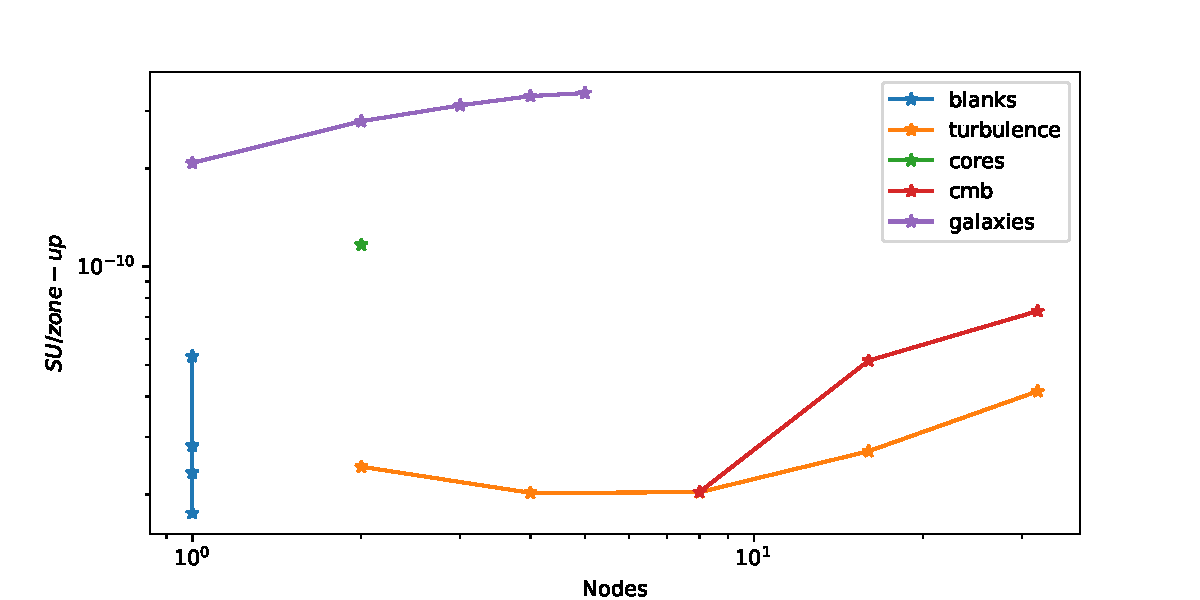
\includegraphics[width=0.99\textwidth]{figs/g47_zoneup.pdf}
\caption[ ]{The cost per zone-update for each of our simulation suites.  
Each fiducial simulation is nearly identical to the target production
simulations.
    }

\label{fig.scaling} \end{center} \end{figure}



\bibliographystyle{apj}
\bibliography{apj-jour,ms.bib}  % looks in ms.bib for bibliography info

\end{document}  


        %dcc todo 2022 
%%\input{SUs}            %dcc todo 2022
%%\input{PriorWork}      %dcc todo 2022 
%%\input{OtherStuff}     %dcc todo 2022

%\appendix
%\include{ appendix file}


\bibliographystyle{apj}
\bibliography{apj-jour,ms}  % looks in ms.bib for bibliography info
%\bibliography{apj-jour,ms}  % looks in ms.bib for bibliography info

\end{document}  


